\section{Procedure and Analysis}

\subsection{Initiation and characteristics of the laser diode}

After switching on the laser diode and the thermoelectric cooler, we controlled the progression and the coherence of the laser beam and verified the correct position of the lenses, so that the beam focused on the detector of the photodiode. We did this by using an infrared display unit and a white piece of paper in order to be able to see the actual progression of the beam.\\

We then turned on the photodiode and the preamplifier, which we set to DC and the gain to 40 dB. We installed the etalon into the optical path and set it perpendicular to the beam. The laser was modulated by a sawtooth voltage in order to be able to see a few wavelength-peaks of the etalon.\\

In the first part of this measurement, the current of the diode was held at a constant value of $I = (35.1\pm 0.3)\ mA$ while the temperature was varied from $34.0^\circ C$ to $36.5^\circ C$. We measured the scrolling of the peaks in dependence of the temperature.
In the second part of the measurement, we held the temperature constant at a value of $T=(34.7 \pm 0.2)\ ^\circ C$ and changed the current from 20.4 to 36.7 mA.
Our measurements were okay, but left room for improvement, which we did in the second week, with the following adjustments:\\

\begin{center}
\begin{tabular}[H]{l l c}
Constant Temperature & \\
Temperature & $T=34.7 ^\circ C$\\
Current & $I = 54.0 \dots 69.0\ mA$\\
 & \\
Constant Current & \\
Laser Current & $I = 64.4 mA$\\
Temperature & $T=32.3 \dots 33.65\ ^\circ C$\\
\end{tabular}
\end{center}

For both measurements, we followed one peak and measured its position in dependence of the current or the temperature of the laser diode. We used the distance of the different peaks to calculate the calibration factor $f$ between the relative position $\Delta t$ and the relative frequency $\nu$ of the peak. It is given by

$$ f = \frac{FSR}{\Delta t} \ \ \ \ \ \text{with the error}\ \ \ \ \ \frac{s_f}{f} \approx \frac{s_{FSR}}{FSR} = 3.00 \cdot 10^{-3} $$

where FSR is the free spectral range of the etalon, whose numerical value is $FSR = (9924 \pm 30)\ MHz$. The error $s_t$ is negligible. The frequency is the given by:

$$\nu = f\cdot t \ \ \ \ \ \text{with the error}\ \ \ \ \ \frac{s_\nu}{\nu} \approx \frac{s_f}{f} = 3.00 \cdot 10^{-3} $$

\subsubsection{Constant Temperature}

By measuring the distance between two peaks we were able to calculate the calibration factor between time and frequency.

$$f = (70.886 \pm  0.214) \frac{MHz}{\mu s} $$

We then were able to plot the relative frequency in dependence of the variation of the laser current and by linear regression find out their relation.

\begin{figure}[H]
\centering 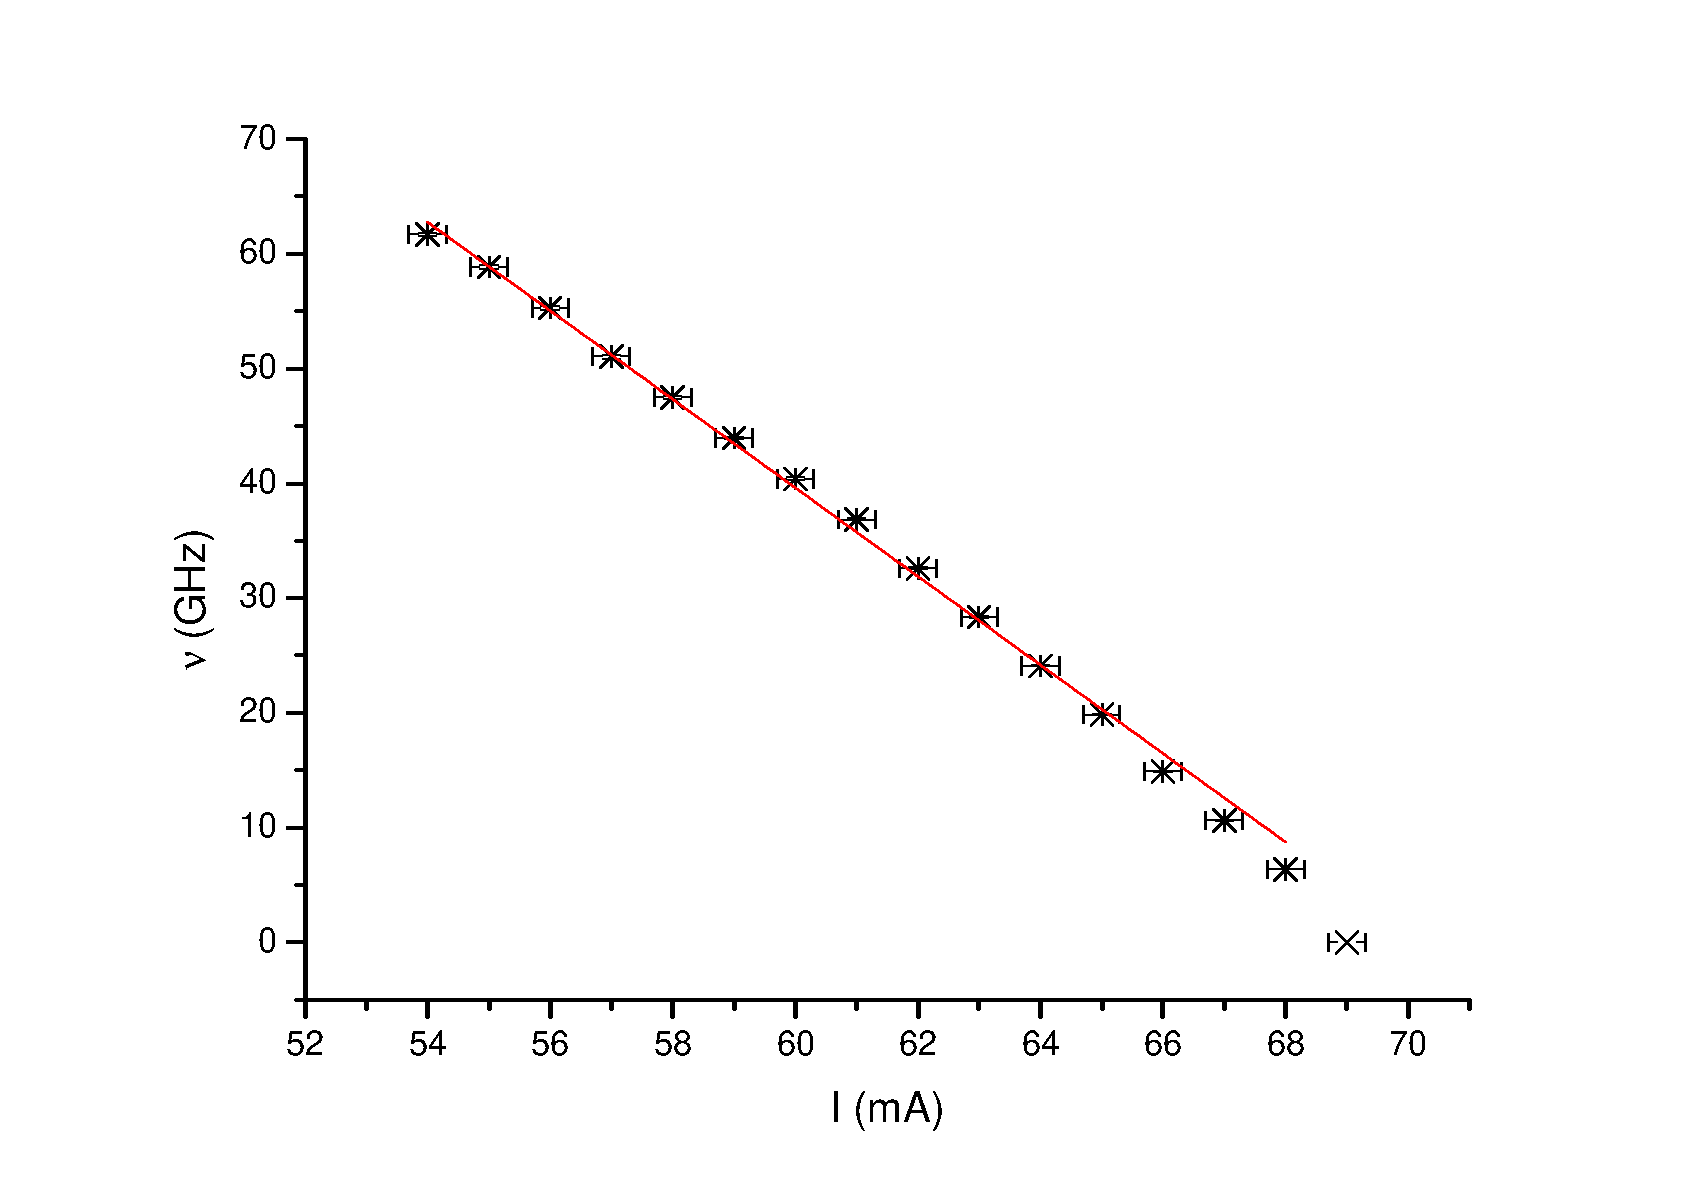
\includegraphics[width=0.9\textwidth]{BilderAusw/T_fest.pdf}
\caption{Variation of the laser current with constant temperature}
\end{figure}

As one can see, the slope is negative, which means that by increasing the current, the light emitted by the laser has a lower frequency. We find that the slope is

$$ a = (-3.858 \pm 0.056)\ \frac{GHz}{mA}$$

which is the conversion factor between the frequency $\nu$ of the laser light and the current $I$ of the diode.

\subsubsection{Constant Current}

The calibration gave us the same conversion factor as before, i.e.

$$f = (70.886 \pm  0.214) \frac{MHz}{\mu s} $$

and we plotted the relative frequency in dependence of the temperature of the laser.

\begin{figure}[H]
\centering 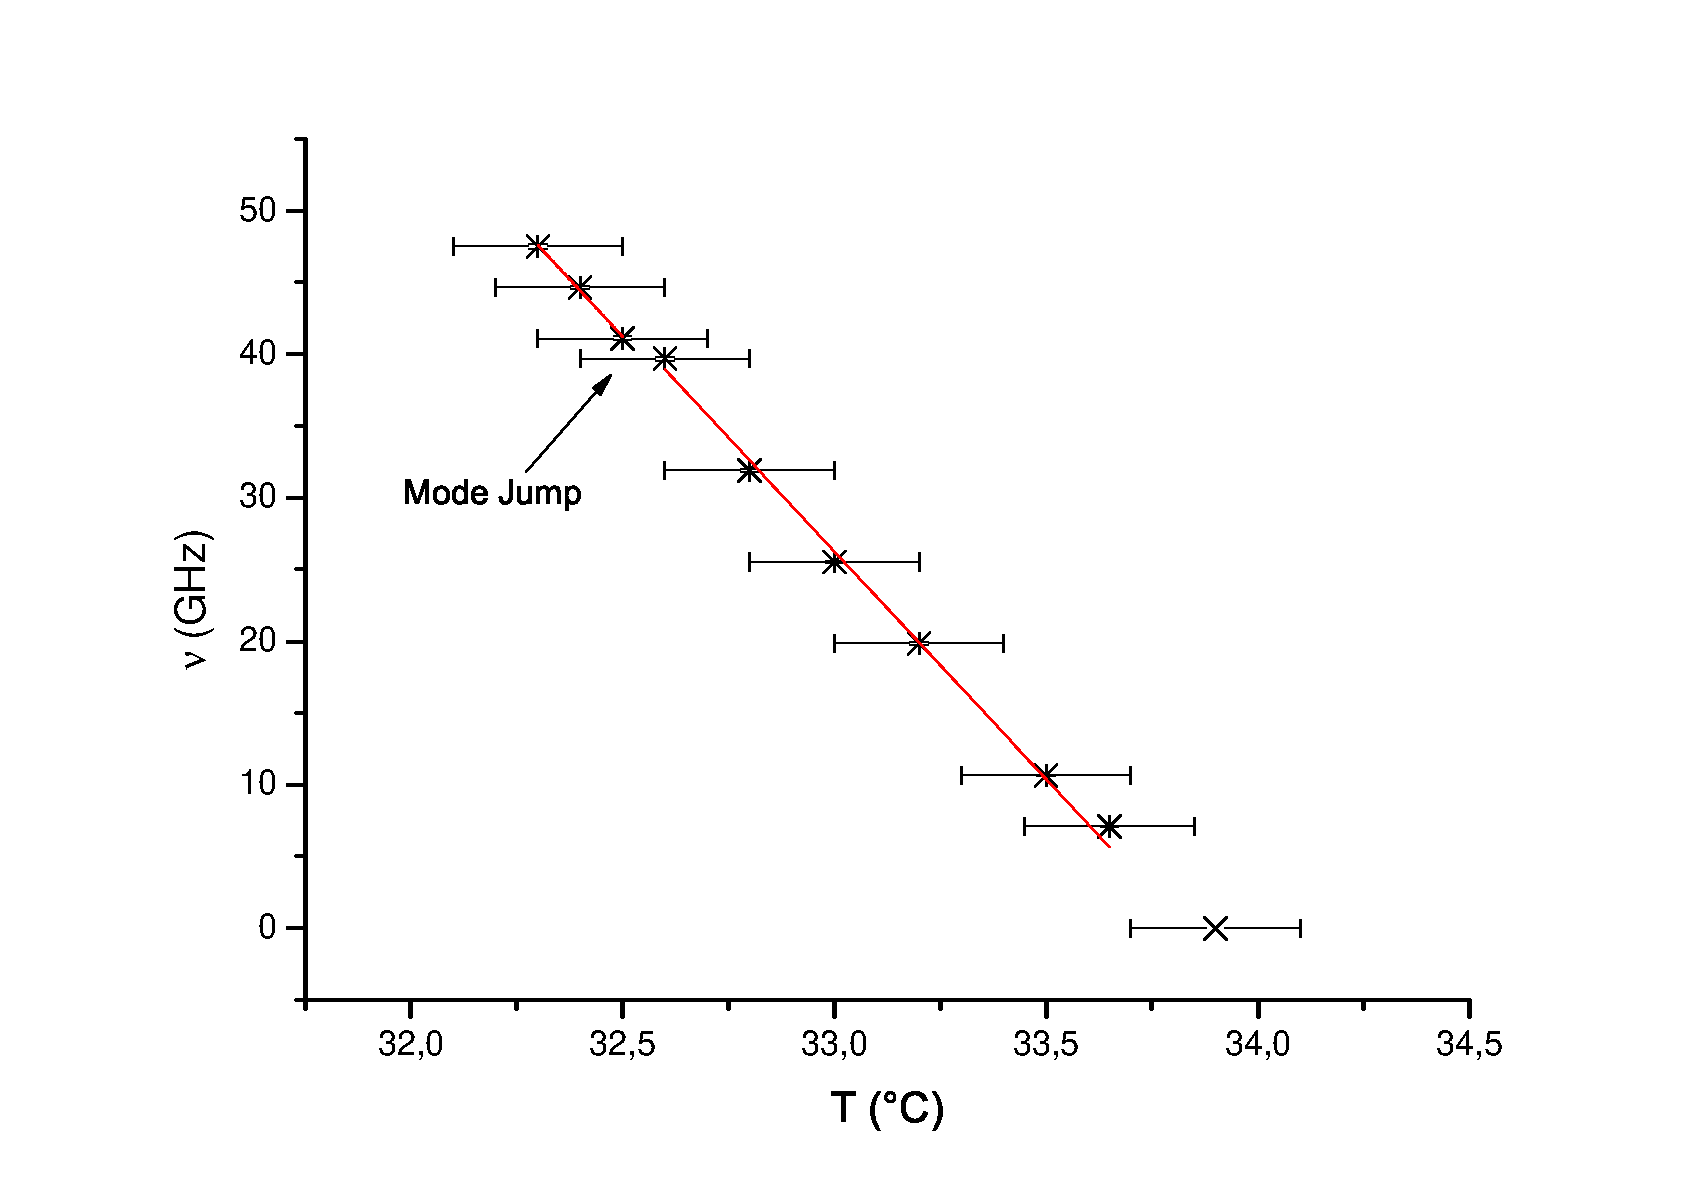
\includegraphics[width=0.9\textwidth]{BilderAusw/I_fest.pdf}
\caption{Variation of the laser temperature with constant current}
\end{figure}

Here, one is also able to see, that with increasing temperature, the frequency decreases. Also, we can see a mode jump near 32.5$^\circ C$. Both parts were fitted by a straight line, and the slopes are as follows:

\begin{center}
\begin{tabular}[H]{l l}
First Slope & $a_1 = (-31.81 \pm 2.05) \frac{GHz}{^\circ C}$\\
Second Slope & $a_2 = (-31.70 \pm 1.12) \frac{GHz}{^\circ C}$\\
\end{tabular}
\end{center}

For the rest of the measurements, we always used temperatures superior to 32,5 $^\circ C$, so the second slope is the one relevant as a conversion factor between temperature and frequency.

\subsubsection{Results}

\begin{tabular}[H]{l c}
Conversion Factors: & \\
Frequency-Current & $\Delta\nu = \Delta I \cdot (-3.858 \pm 0.056)\ {Ghz}/{mA}$\\
Frequency-Temperature & $\Delta\nu = \Delta T \cdot (-31.70 \pm 1.12)\ {Ghz}/{^\circ C}$\\
\end{tabular}


\subsection{Hyperfine Structure}

We installed the Rubidium cell into the optical path and removed the etalon. The laser diode was modulated by a triangular voltage with a peak-to-peak difference of $\sim 200\ mV$, and the temperature was set to $T = (34.6 \pm 0.2)^\circ C$, as described in the instructions. The preamplifier was set to AC from now on. However, with these adjustments we weren't able to find the hyperfine structure of the Rubidium atoms. Furthermore, the current of the laser diode wasn't able to surpass 35 mA and the preamplifier of the photodiode  was overcharged. We then tried different adjustments and installed a neutral filter (\emph{D 4,3}) into the optical path. The new adjustment was:\\

\begin{center}
\begin{tabular}[H]{l c}
Temperature & $T=34.4 ^\circ C$\\
Peak-to-Peak Voltage & $U_{pp} = 134\ mV$\\
\end{tabular}
\end{center}

We were then able to see the hyperfine structure at a current of $I = (62.9 \pm 0.3)\ mA$. With the same adjustments, we did another calibration. For this, however, we had to remove the filter, because the peaks weren't visible else. This measurement was also redone in the second week with the following adjustments:

\begin{center}
\begin{tabular}[H]{l c}
Temperature & $T=34.5 ^\circ C$\\
Peak-to-Peak Voltage & $U_{pp} = 4\ V$\\
Laser Current & $I = 63.9 mA$\\
\end{tabular}
\end{center}

The measurements were even better this time.

\subsection{Double Resonance}
\subsection{Spin Precession}
\subsection{Relaxation Time (Dehmelt)}
\subsection{Relaxation Time (Franzen)}















